\documentclass[10pt,a4paper]{article}

%double si on veut une version prof et une version élève. simple si on veut une seule version.
\newcommand{\buildmode}{double}

\InputIfFileExists{version.tex}{}{}
% Version (définie par le script)
\providecommand{\version}{eleve}

\usepackage{feuilleexo}
\usepackage{schemaevolution}

%%%à modifier à chaque fois

\renewcommand{\niveau}{SBM 2A}
\renewcommand{\chapitre}{Généralités sur les fonctions}
\renewcommand{\numchap}{0.2} 
\renewcommand{\theme}{Fontions}

\begin{document}


%\legendeicones

\vspace{-0.3cm}

\begin{prerequis}
\begin{itemize}
    \item Savoir résoudre une équation simple.
    \item Savoir lire et exploiter un graphique
    \item Maîtriser les concepts liés aux fonctions affines
\end{itemize}

\end{prerequis}

\prof{
    Objectif : \begin{itemize}
        \item Savoir ce qu'est une fonction, les comprendre comme un modèle prédictif de la réalité grâce à des modélisations par des fonctions affines.
        \item Maîtriser le concept de variations d'une fonctions et de tangente. Comprendre le coefficient directeur comme une quantification de la pente. Objectif : intrduire le nombre dérivé.
    \end{itemize}
}
\begin{multicols}{2}

    \section{Rappels sur les fonctions}
\begin{exo}[][]
On a mesuré en continu pendant quatre heure, la concentration \(C\) d'un médicament dans le sang d'un patient. a fonction \(C\) est représentée ci-dessous.

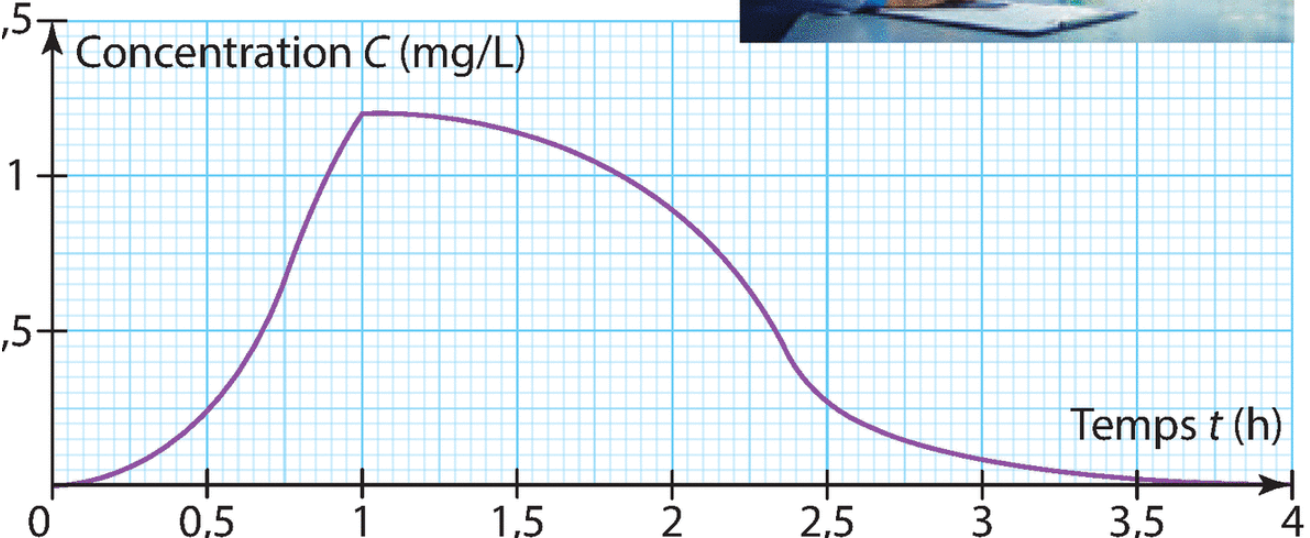
\includegraphics[width=0.4\textwidth]{concentration_sang.png}

\begin{enumerate}
    \item Utiliser le graphique pour répondre aux questions suivantes :\\
    \begin{tabular}{|p{0.2\textwidth}|p{0.2\textwidth}|}
    \hline
    Question & Réponse \\
    \hline 
    Quelle était la concentration au bout de 2 h ? & \\ \hline
    Au bout de combien de temps la concentration était-elle de 0,5mg/L ? & \\ \hline
    Quand est-ce que la concentration augmente ? & \\ \hline
    Quel est la concentration la plus haute ? & \\ \hline
    \end{tabular}

    \item À l'aide de vos réponses, recompléter le tableau à l'aide du vocabulaire sur les fonctions
        \begin{tabular}{|p{0.2\textwidth}|p{0.2\textwidth}|}
    \hline
    Question & Réponse \\
    \hline 
    Quelle est l'image de 2 par la fonction \(C\) ? // Que vaut \(C(2)\) & \\ \hline
     & \begin{minipage}{0.1em}
        \vspace{1.5cm}
     \end{minipage} \\ \hline
     & \begin{minipage}{0.1em}
        \vspace{1.5cm}
     \end{minipage} \\ \hline
     & \begin{minipage}{0.1em}
        \vspace{1.5cm}
     \end{minipage} \\ \hline
    \end{tabular}

    \item Répondre aux questions suivantes :\begin{enumerate}
        \item Que vaut \(C(1)\) ?
        \item Résoudre l'équation \(C(x) = 1\)
        \item Quelle est l'image de 4 ?
        \item Quel est le sens de variations de \(C\) sur l'intervalle \([2\ ;\ 3,5]\) ?
    \end{enumerate}
\end{enumerate}
\end{exo}

\begin{exo}[][]
    On considère la fonction \(f\) définie par \(f(x)=x^2-2x+3\). 


    \begin{enumerate}
    \item Complétez le tableau de valeurs suivant.
    
    \begin{center}
        \renewcommand{\arraystretch}{1.5} %donne la distance entre les lignes%
        \setlength{\tabcolsep}{0.3cm} %donne la distance entre les colonnes%
        \begin{tabular}{|c|c|c|c|c|c|c|}
        \hline
        \(x\) & -1 & 0 & \(\frac{1}{2}\) & 1 & 2 & 3  \\
        \hline
        \(f(x)\) &  &  &  &  &  &  \\
        \hline
        \end{tabular}
    \end{center}
    
    \item À l'aide du tableau, tracer la courbe représentative de la fonction.
    
    \hspace{-1cm}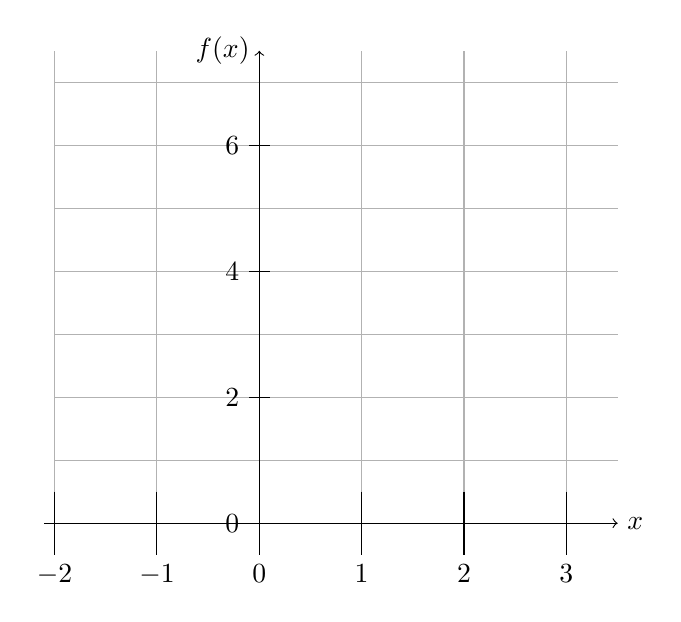
\begin{tikzpicture}[yscale=0.8, xscale=1.3]
        \draw[step=1.0,black!30!white,thin] (-2,0) grid (3.5,7.5);
        \draw[->] (-2.1,0) -- (3.5,0) node[right] {\(x\)};
        \draw[->] (0,-0.5) -- (0,7.5) node[left] {\(f(x)\)};
        \foreach \x in {-2,...,3} \draw (\x,0.5) -- (\x,-0.5) node[below] {\(\x\)};
        \foreach \y in {0,2,...,6} \draw (0.1,\y) -- (-0.1,\y) node[left] {\(\y\)};
    \end{tikzpicture}
    \end{enumerate}
\end{exo}

\section{Fonctions affines}

\prof{
    Faire un rappel sur les fonctions affines ici. Si ce n'est pas maîtrisé (on peut éventuellement leur demander), leur faire tracer une ou deux fonctions affines et faire retrouver la fonction affine à partir d'une droite.
}
\begin{exo}[][ccf]
    On cherche à étudier l’évolution de la température à l’intérieur d’une serre.  
Un système de chauffage est testé, modélisé par la fonction $s$.  
Le graphique ci-dessous représente ces fonctions :

\begin{center}
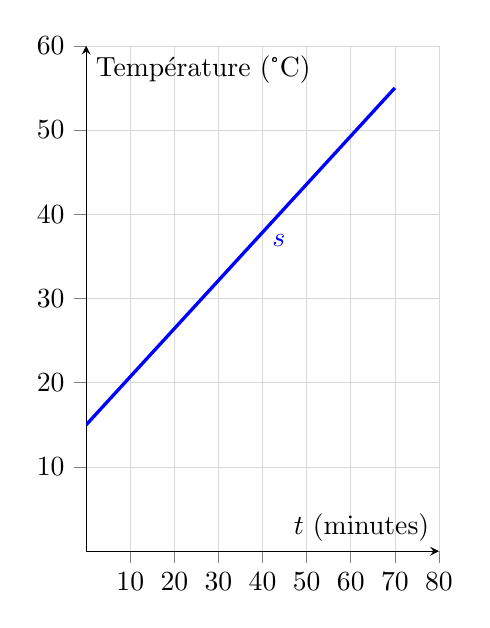
\begin{tikzpicture}
  \begin{axis}[
    width=0.5\textwidth, height=8cm,
    axis x line=middle, axis y line=middle,
    xmin=0, xmax=80, ymin=0, ymax=60,
    xtick={0,10,20,30,40,50,60,70,80},
    ytick={0,10,20,30,40,50,60},
    grid=both, grid style={line width=.1pt, draw=gray!20},
    major grid style={line width=.2pt,draw=gray!30},
    xlabel={$t$ (minutes)}, ylabel={Température (°C)},
    tick align=outside
  ]

  % première fonction s : démarre à 15°C, finit à 55°C en 70 minutes
  \addplot[blue, very thick] coordinates {(0,15) (70,55)};
  \node[anchor=south west, blue] at (axis cs:40,35) {$s$};

  \end{axis}
\end{tikzpicture}
\end{center}
\begin{enumerate}
    \item \begin{enumerate}
        \item Déterminer le coefficient directeur et l'ordonnée à l'origine de la droite.
        \item En déduire une expression de \(s(t)\)
        \item Quelle sera la température de la serre au bout de 2h de chauffe ?
        \item Au bout de combien de temps la température atteindra-t-elle 70°C ?
    \end{enumerate}
\end{enumerate}
\end{exo}

\begin{exo}[][ccf]
    \textbf{Régression affine -- Temps de séchage d'un produit}

    Dans un laboratoire, on étudie le temps nécessaire pour sécher un échantillon en fonction de la température de séchage.

    On réalise plusieurs expériences et on obtient les résultats suivants :

    \begin{center}
        \begin{tabular}{|p{2.5cm}|*{7}{c|}}
            \hline
            Température \(x\) (en \(^\circ\mathrm{C}\))
            & 40 & 45 & 50 & 55 & 60 & 65 & 70 \\
            \hline
            Temps de séchage \(y\) (en min)
            & 82 & 74 & 68 & 61 & 55 & 50 & 44 \\
            \hline
        \end{tabular}
    \end{center}

    \begin{enumerate}
        \item Représenter le nuage de points associé à cette série statistique dans un repère.

        \item Que peut-on dire de l'allure du nuage de points ?

        \item À l'aide de la calculatrice, déterminer une équation de la droite d'ajustement affine de \(y\) en \(x\), obtenue par la méthode des moindres carrés.

        On donnera une valeur approchée des coefficients au centième.

        On pourra noter cette équation :
        \[
            y=ax+b.
        \]

        \item À l'aide de l'ajustement affine, estimer le temps de séchage nécessaire pour une température de \(57\,^\circ\mathrm{C}\).

        \item Le laboratoire souhaite que le temps de séchage soit inférieur à \(45\) minutes.

        À l'aide de l'équation de la droite d'ajustement, estimer la température minimale nécessaire pour atteindre cet objectif.

        \item La droite d'ajustement est-elle nécessairement pertinente pour prévoir le temps de séchage à \(100\,^\circ\mathrm{C}\) ?
        
        Justifier.
    \end{enumerate}
\end{exo}

\section{Tableaux de signe}

\begin{exo}[][]
    Dresser les tableaux de signe des fonctions affines suivantes :
    \begin{tasks}(2)
        \task \(f(t) = 7t+14\)
        \task \(g(x) = -2x+5\)
        \task \(h(x) = x-4\)
        \task \(i(x) = -x-\dfrac{2}{3}\)
    \end{tasks}
\end{exo}

\prof{
    Obligation de justifier le tableau de signe par  un schéma. Ce sera le cas pour l'interro
}

\begin{exo}[][]
    On considère les fonction affines \(f\) et \(g\) définies par \(f(x) = x-4\) et \(g(x) = x+1\).\\
    On considère également la fonction \(m\) définie par \(m(x)=2x^2-6x-8\)
    \begin{enumerate}
        \item Démontrer l'égalité suivante : \(-2(x-4)(x+1) = 2x^2-6x-8\).
        \item En déduire le tableau de signe de la fonction \(m\). Vous pourrez vous aider des tableaux de signe de \(f\) et \(g\).
        \item Tracer la fonction \(m\) entre -2 et 5. Les résultats sont-ils cohérents ?
    \end{enumerate}
\end{exo}

\prof{
    \begin{itemize}
        \item Est-ce que c'est nécessaire de faire tracer la courbe ? Ça prend du temps.
        \item On n'a pas revu comment tracer un tableau de signe à l'aide d'une représentation graphique, est-ce que ça pose problème ?? (C'est pour ça que j'ai rajouté la question 3).
    \end{itemize}
}

\begin{exo}[][]
    On considère la fonction \(g\) définie par \(g(x) = 3x^-9x+6\)
    \begin{enumerate}
        \item Développer l'expression \(3(x-2)(x-1)\)
        \item En déduire le tableau de signe de \(g\)
    \end{enumerate}
\end{exo}

\begin{exo}[][]
    On considère la fonction \(h\) définie par \(h(t) = t^2+2t+1\)
    \begin{enumerate}
        \item Développer l'expression \((t+1)^2\)
        \item En déduire le tableau de signe de \(h\)
    \end{enumerate}
\end{exo}
\end{multicols}
\end{document}
